%File: formatting-instruction.tex
\documentclass[letterpaper]{article}
\usepackage{aaai}
\usepackage{times}
\usepackage{helvet}
\usepackage{courier}
\usepackage{url}
\usepackage{graphicx}
\usepackage{subcaption}
\graphicspath{{Figures/}}
\frenchspacing
\setlength{\pdfpagewidth}{8.5in}
\setlength{\pdfpageheight}{11in}
\pdfinfo{
	/Title (Insert Your Title Here)
	/Author (Put All Your Authors Here, Separated by Commas)}
\setcounter{secnumdepth}{0}  
\begin{document}
	% The file aaai.sty is the style file for AAAI Press 
	% proceedings, working notes, and technical reports.
	%
	\title{There is a pot of gold, you just don't see it: \\ Applying Rainbow to partially observable environments}
	\author{David Slayback\\
		Northeastern University College of Computer and Information Science\\
		440 Huntington Ave, No. 202\\
		Boston, Massachusetts 02115\\
	}
	\maketitle
	\begin{abstract}
		\begin{quote}
			Recent breakthroughs in deep reinforcement learning have led to AI solutions to many previously untenable games and environments. ViZDoom, an interface to the popular first person shooter (FPS) DOOM, is a particularly informative environment because of the partial observability of the state and potential complexity of the actions. This paper details an attempt to apply Rainbow, a reinforcement learning (RL) algorithm combining several improvements to Deep Q-Networksv (DQN), to different scenarios within the ViZDoom environment. Preliminary results reveal the difficulty of the environment and offer insights into future directions for improving agent performance.
		\end{quote}
	\end{abstract} 
	
	\section{Introduction}
	
	In the past decade, with new access to data and computational power, artificial intelligence (AI) researchers have made enormous strides. Deep learning (DL), a type of machine learning once considered computationally intractable, has revolutionized our approach to many problems. Deep neural networks (DNNs) provide a generalizable alternative to previous domain-specific solutions. Reinforcement learning (RL) provides a framework with which an AI could potentially learn anything.
	
	A natural application of these techniques has been to games. Games provide a perfect simulator in which researchers can test new AI techniques. Many of the recent advances have focused on old Atari environments because of their relative simplicity and ease of computation. However, more modern games may offer comparable complexity to real-life environments while maintaining the consequence-free and data collection friendly properties. 
	
	As such, in this paper I set out to apply Rainbow, an algorithm combining many recent advances in deep reinforcement learning, to the more complex, partially-observable environment of VizDoom.
	
	\section{Background}
	
	Reinforcement learning (RL) is a method by which some \textit{agent} can learn to act in an unknown \textit{environment} to maximize some goal expressed via \textit{rewards}. RL is unique in that the agent does not need to be told \textit{how} to act; rather, it learns through trial-and-error by encountering rewards as it acts and attempting to choose actions which maximize future rewards.
	
	\subsection{RL Terminology}
	 
	 The interaction of the agent and the environment is formalized as a Markov Decision Process (MDP). An MDP is defined by a tuple $\langle S, A, T, R, \gamma \rangle$ where:
	 \begin{itemize}
	 	\item $S$ is the set of possible states of the environment
	 	\item $A$ is the set of possible actions of the agent
	 	\item $T$ is the transition function $T(s,a,s')$ giving the probability of reaching each state $s'$ from state $s$ when taking action $t$
	 	\item $R$ is the reward function $R(s,a)$ giving the reward of taking action $a$ in state $s$
	 	\item $\gamma$ is a discount factor applied to future rewards
	 \end{itemize}
 	
 	At each timestep $t\in \tau$ (where $\tau$ is the end time), the agent takes an action $a_t$ from start state $s_t$. The state changes to $s_{t+1}$, and the agent receives an immediate reward $r_{t+1}$. The agent chooses it's action based on a \textit{policy} $\pi (a_t|s_t)$ which gives the probability of taking action $a_t$ in state $s_t$. The objective of reinforcement learning is to achieve an optimal policy $\pi^*$ which maximizes the reward the agent accumulates in the environment (i.e., the \textit{return}, $G_t=\sum_{n=0}^{\infty}\gamma^k_tR_{t+k+1}$). 
 	
 	In value-based reinforcement learning, the agent learns $\pi$ by determining the \textit{Q-value} of its actions, where $Q^\pi(s,a)$ is the expected return of taking action $a$ in state $s$ if the agent chooses future actions based on policy $\pi$. It then derives a policy that takes the actions with the highest value, updating values as it encounters rewards. In \textit{TD-learning}, the q-value is updated after each action, minimizing the difference between the \textit{TD-target} (i.e., the currently estimated value of the state) and the combination of immediate reward and next state value seen (known as \textit{TD-error}).
 	
 	\subsection{Large state spaces}
 	
 	One problem with this formalism is computational. In simple environments with few states and actions, an agent can store and calculate each $Q(s,a)$. In more complex environments, however, if the agent is even able to store all possible $Q(s,a)$, the number of actions it must take to accurately calculate them increases exponentially.
 	
 	This issue can be solved by replacing the tables with DNNs, allowing the agent to learn reduced approximations of policies and values. Specifically, in the original DQN architecture \cite{mnih2015human} used for Atari games, the agent has a network that computes the Q-value for any input combination of pixels from the game frames. This network is parameterized by weights $\theta$ ($\widehat{\theta}$ being a periodic copy of the weights), such that the loss can be defined as:
 	\begin{equation}
	 	(R_{t+1}+\gamma_{t+1}max_{a'}q_{\widehat{\theta}}(s_{t+1}, a')-q_{\theta}(s_t, a_t)
 	\end{equation}
 	Training an accurate DQN is data-intensive, but can leverage a \textit{replay buffer} to reuse the agent's experiences and learn \textit{off-policy} (i.e., without taking actions in the environment). This buffer of transitions $(s_t, a_t, r_{t+1}, \gamma_{t+1}, s_{t+1})$ can be sampled in random batches to provide additional training at only the cost of computational time.
 	
 	\subsection{Partial Observability}
 	
 	Another problem with the original formalism is sensory. In most environments, it's unrealistic for the agent to have access to the full state of the environment. Rather, the agent receives \textit{observations} from its sensors in the form of camera images, communications, or other modalities. An extended formalism to capture this is known as a Partially Observable MDP (POMDP). A POMDP is an extended MDP defined by a tuple $\langle S, A, T, R, \Omega, O, \gamma \rangle$, where:
 	\begin{itemize}
 		\item $\Omega$ is the set of possible observations $o$
 		\item $O$ is the conditional probability function $O(o|s',a)$ specifying the probability of the agent observing $o$ after taking action $a$ and reaching environment state $s'$
 	\end{itemize}
 
 	At each timestep $t\in \tau$, the environment is in state $s_t$, the agent takes action $a_t$ and receives observation $o_t+1$ and reward $o_t+1$. The environmental state may change, but the agent doesn't know. Rather, the agent determines a policy either directly from observation $\pi(a_t|o_t)$ or by developing a belief about the state $s$ from its observations ($\pi(a_t|b_t)$ where $b_t$ is a \textit{belief} about the current state). 
 	
 	However, a single observation may not be sufficient to determine an optimal action or belief, so these are often conditioned on some history of actions, observations, and rewards $h$. Maintaining such a history is itself a problem, since it is difficult to know which experiences are relevant and impossible to store all of them.
 	
 	\subsection{Deep Recurrent Q-Networks}
 	
 	One potential solution to this is to approximate the history in the same way that DQN approximated the Q-values. Deep Recurrent Q Networks (DRQNs) are an extension to DQN that incorporate \textit{recurrent} network layers\cite{hausknecht2015deep}. A recurrent network layer is any layer whose output is conditioned on previous inputs. What outputs are conditioned on is known as the \textit{hidden state} of the layer and serves as an approximate memory.
 	
 	Thus, by incorporating recurrent layers, a DRQN is able to infer the state from temporally extended inputs, and so its calculated $Q(o,a)$ can more accurately reflect sequences of events. The original DQN approximated this by providing input as a sequence of 4 frames*.
 	
	 
	
	\section{Related Work}
	
	The primary motivation behind this paper was Rainbow, a paper which combined several improvements to DQN\cite{hessel2017rainbow}. Specifically, Rainbow applies:
	\begin{itemize}
		\item \textbf{Double Q-Learning}: Using a target network to reduce maximization bias\cite{hasselt2010double}. Chooses the action with the policy network, but evaluates the chosen action with the target network. Loss:
		
		\begin{equation}
			(R_{t+1}+\gamma_{t+1}q_{\widehat{\theta}}(s_{t+1}, argmax_{a'}q_{\theta}(s_{t+1}, a')-q_{\theta}(s_t, a_t))^2
		\end{equation}
	
		\item \textbf{Prioritized Replay}: Weighting experiences based on their difference from expected value\cite{schaul2015prioritized}. Sample transitions with probability proportional to the last encountered \textit{TD-error} at that transition.
		\begin{equation}
			p_t \propto |R_{t+1} + \gamma_{t+1}max_{a'}q_{\widehat{\theta}}(s_{t+1}, a')-q_{\theta}(s_t, a_t)|^\omega
		\end{equation}
		\item \textbf{Dueling Networks}: Dividing the output of a network into two streams corresponding to the value of a state and the relative advantage of taking an action\cite{wang2015dueling}. The output is the value plus the best action minus the mean over all actions.
		
		\item \textbf{Multi-step Learning}: Calculating the return of multiple future steps rather than just the immediate reward and expected value of the next state\cite{sutton2018reinforcement}. The n-step return is:
		
		\begin{equation}
			R_t^{(n)}=\sum_{k=0}^{n-1}\gamma_t^{(k)}R_{t+k+1}
		\end{equation}
		
		
		\item \textbf{Distributional RL}: Maintaining a distribution of expected Q-values rather than a single one\cite{bellemare2017distributional}. Goal is to minimize the  KL divergence between the distribution $d_t$ and the target distribution $d_t'$
		
		\item \textbf{Noisy Nets}: Replacing $\epsilon$-greedy exploration (i.e., taking a random action with probability $\epsilon$) with implicit exploration in the form of injected noise during training\cite{fortunato2017noisy}. In place of a linear layer $y=b + Wx$: 
		
		\begin{equation}
			y = (b+Wx)+(b_{noisy} \odot \epsilon^b + (W_{noisy}\odot \epsilon^w)x)
		\end{equation}
	\end{itemize}
	Rainbow and its ablations were tested extensively on the Atari environment in an attempt to determine which improvements made the biggest difference and explain the potential advantages of each. They concluded that prioritized replay and multi-step learning were the most impactful additions, but that the impacts of all the improvements were dependent on the environment chosen. Thus, it would be of interest to see how these improvements interact with more complex, partially-observable environments. 
	
	The other motivation was to leverage the VizDoom environment. VizDoom is a doom-based AI research platform specifically tailored to deep reinforcement learning\cite{kempka2016vizdoom}. As such, it has inspired both an annual AI deathmatch competition\cite{wydmuch2018vizdoom} and several papers. Among these is Chaplot and Lample's Arnold \cite{chaplot2017arnold}, an AI which combines DRQN navigation and DQN shooting and which won the 2017 competition. Arnold forms the primary basis for this paper's AI architecture.
	
	\section{Project Description}
	
	This project consisted of 3 main parts.
	\begin{itemize}
		\item Implement the algorithms from Rainbow for a DRQN-based agent
		\item Develop a scenario in VizDoom 
		\item As in Rainbow, permute which algorithms are used for the agent and observe how the permutation affects training
	\end{itemize}

	For the first part, all networks are implemented in PyTorch. At first, I decided to re-use Arnold's architecture, found in their github \cite{lample2018}. As it had won a full deathmatch competition, it seemed that the architecture they used must have been a reasonable choice for the environment. I made one major change, though. Originally, Arnold took advantage of the game providing labels that flagged whether different entities were on the screen (e.g., flagging that an enemy is in view). They only used this during training, but it seemed an unfair advantage, so I removed it. The architecture is as follows:
	\begin{itemize}
		\item Each game frame is processed to 3x60x108 pixels. The authors noted that both color and a wide aspect ratio seemed to speed training.
		\item This input goes through two convolutional layers (with ReLU activation and batch normalization)
		\item Additionally, the game variables for health and ammo are processed through an embedding layer (32 dimensions for each variable)
		\item Both outputs are fed into a 1-layer LSTM with 512 hidden units
		\item The LSTM's output is mapped to actions through a linear layer
		\item For experiments using the dueling architecture, the final linear layer was replaced with two linear layers to serve as value and advantage streams. Their outputs were fused together as mentioned above.
	\end{itemize} 

	\begin{figure}[h!]
		\centering
		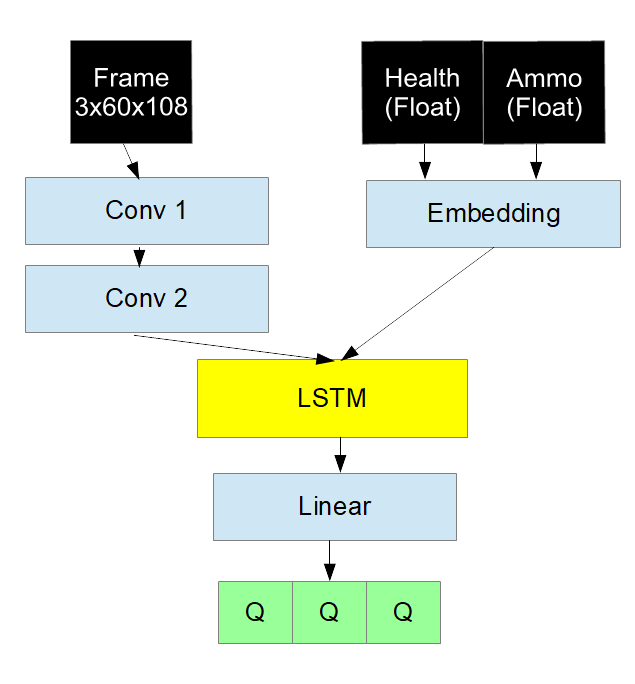
\includegraphics[width=0.5\textwidth]{Arch.png}
		\caption{Arnold-inspired architecture}
		\label{fig:ArnoldArch}
	\end{figure}

	Additionally, I adapted the code for prioritized replay and n-step learning from a different repository\cite{kaixhin2018}. For this instantiation, I did not implement distributional RL due to the complexity.
	
	After this modified architecture showed poor results, I wrote an entirely new version for a basic 1-frame DQN that heavily borrowed from SLM lab\cite{kenggraesser2017slmlab} and a series of pytorch tutorials\cite{fettes2018}. In this case, I was able to adapt all 6 Rainbow algorithms.
	
	When the new architecture also showed poor results, I extended it to a stacked-frame DQN similar to the original Atari paper. 
	
	For the second part, I had originally intended to define my own scenario. VizDoom provides a number of useful prebuilt scenarios, but I felt that most of them would be too simple. As it became clear that my agent was failing to learn, I turned back to the original scenarios. The scenario I tested my Arnold reimplementation on is called "Defend the Line", and the scenario I tested the others on is "Defend the Center". Both are described in the experiments section.
	
	For the third part, I attempted to replicate the ablations of the rainbow paper. For each series of experiments, I did a run with the base architecture, with the fully augmented rainbow version, and then one run for each component to be removed in turn. I hypothesized that the VizDoom environment might have a different pattern of impact from these enhancements than the Atari games had. 
	
	My code can be found at \url{https://github.ccs.neu.edu/dtslayback/CS7180-Project}
	 
	\subsection{Experiments}
	
	The scenarios are defined as follows:
	\begin{itemize}
		\item \textbf{Defend the Line}: The agent starts at the end of a hallway with limited ammunition. 3 melee and 3 ranged monsters spawn at the other end. These monsters can initially be killed by 1 shot, but as new ones spawn, they take progressively more damage.
		\subitem Reward: +1 for each kill
		\subitem Actions: Turn left, turn right, attack
		\item \textbf{Defend the Center}: The agent starts in the center of a room with limited ammunition. 3 melee monsters spawn randomly around the agent. All monsters can be killed with 1 shot.
		\subitem Reward: +1 for each kill
		\subitem Actions: Turn left, turn right, attack
	\end{itemize}

	\begin{figure}[h!]
		\centering
		\begin{subfigure}[b]{0.2\textwidth}
			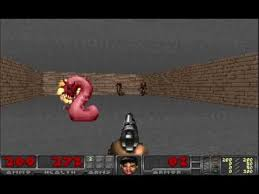
\includegraphics[width=\textwidth]{DefendTheLine.jpg}
			\caption{Defend the Line}
			\label{fig:Line}
		\end{subfigure}
		~ %add desired spacing between images, e. g. ~, \quad, \qquad, \hfill etc. 
		%(or a blank line to force the subfigure onto a new line)
		\begin{subfigure}[b]{0.2\textwidth}
			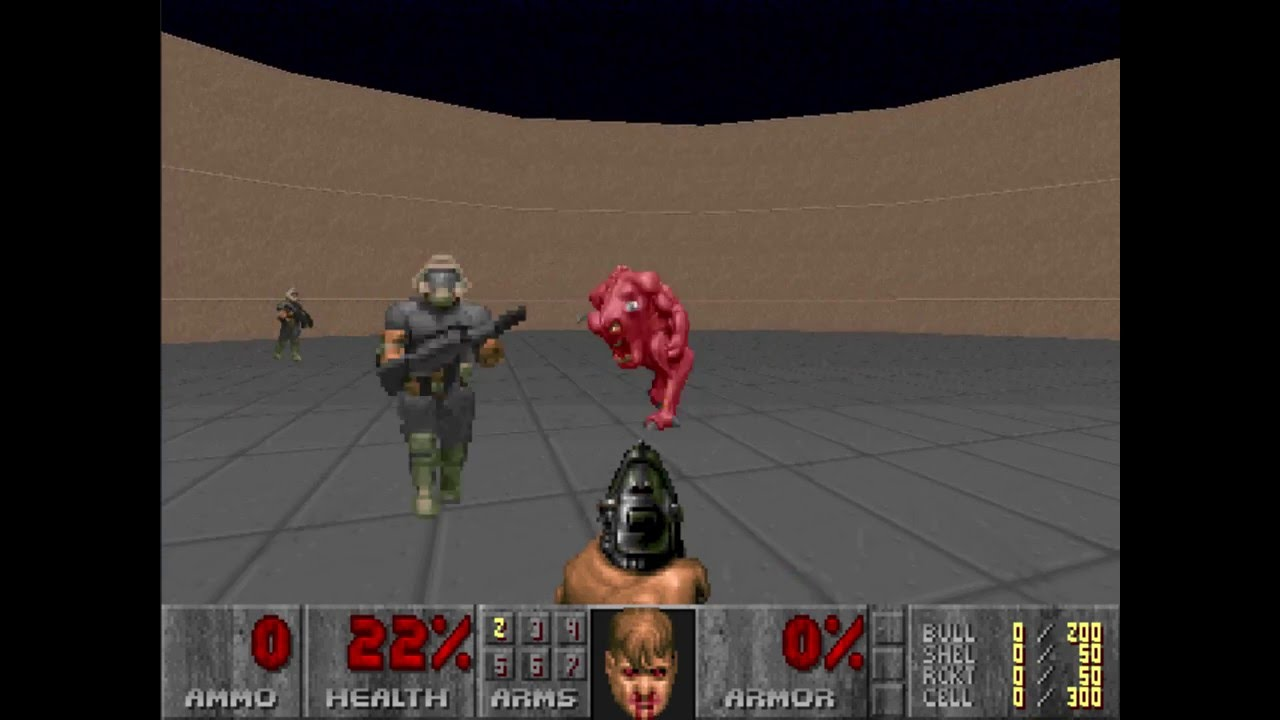
\includegraphics[width=\textwidth]{DefendTheCenter.jpg}
			\caption{Defend the Center}
			\label{fig:Center}
		\end{subfigure}
	\end{figure}

	All implementations of rainbow used the following common parameters, primarily derived from the original paper's choices:
	
	\begin{table}[h]
	\caption{Common Hyperparameters}
	\centering
		\begin{tabular}{c r}
			\hline \hline
			Parameter & Value \\
			\hline
			Start $\epsilon$ & 1.0 \\
			End $\epsilon$ & 0.01  \\
			Steps $\epsilon$ & 250000 \\
			$\gamma$  & 0.99 \\
			Batch Size & 32 \\
			Target update frequency & 1000 \\
			Training Frequency & 4 \\
			Training Start & 80000 \\
			Learning Rate & 0.001 \\
			Optimizer & Adam \\
			$\sigma$ (Noisy) & 0.5 \\
			Priority $\beta$ start & 0.4 \\
			Priority $\beta$ end & 1.0 \\
			Priority $\beta$ steps & 1000000 \\
			Priority $\omega$ & 0.5 \\
			Distributional atoms & 51 \\
			Min dist value & -10 \\
			Max dist value & 10 \\
			Multi-step n & 3 \\
			\hline
		\end{tabular}
	\label{tab:comHyp}
	\end{table}
	
	Additionally, VizDoom offered the option to perform the same action for some number of frames; I used 4 as most VizDoom implementations used that as a good compromise to reduce the number of irrelevant frames.
	
	For the Arnold reimplementation, I chose to use sequences of length 6, updating the network using the outputs from the final 2 frames. For the first DQN, I used 1 frame; for the second, I used 4. 
	
	For the Arnold implementation, I had to reduce the memory capacity from the intended 1 million frames to 250K due to memory constraints. Each ablation trained for 2M frames on the "Defend the Line" scenario. Every 50K frames, the networks were set to evaluation mode (disabling normalization, dropout, and noisy linear layers) and tested on 10 full episodes. The mean episode rewards are reported in the graph below.
	
	For the 1-frame DQN implementation, I used a memory capacity of 500K. However, after the baseline DQN, the remainder of the run crashed. The results are above.
	
	Given the poor results from the 1-frame DQN, I implemented a 4-frame DQN and began the run. To save time, I set it to run for only 500K frames and evaluate every 20K on 20 episodes. Unfortunately, by the time of publication, not all results had come in; the finished ones are reported above. Disappointingly, it demonstrates the same failure to learn.
	
	\begin{figure}
		\centering
		\begin{subfigure}[b]{0.3\textwidth}
			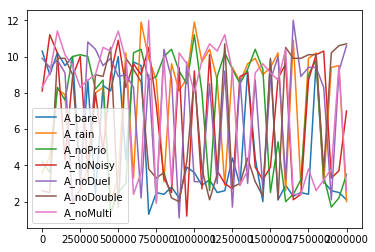
\includegraphics[width=\textwidth]{ArnoldResults}
			\caption{Results of Arnold reimplementation on Defend the Line}
			\label{fig:ArnoldResults}
		\end{subfigure}
		~ %add desired spacing between images, e. g. ~, \quad, \qquad, \hfill etc. 
		%(or a blank line to force the subfigure onto a new line)
		\begin{subfigure}[b]{0.3\textwidth}
			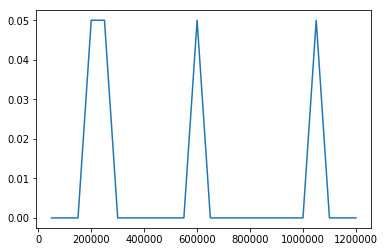
\includegraphics[width=\textwidth]{DQN1Results}
			\caption{1 frame DQN results on Defend the Center}
			\label{fig:DQN1Results}
		\end{subfigure}
		~ %add desired spacing between images, e. g. ~, \quad, \qquad, \hfill etc. 
		%(or a blank line to force the subfigure onto a new line)
		\begin{subfigure}[b]{0.3\textwidth}
			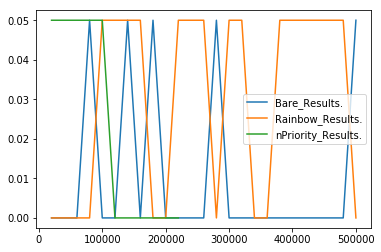
\includegraphics[width=\textwidth]{DQN4Results}
			\caption{14 frame DQN results on Defend the Center}
			\label{fig:DQN4Results}
		\end{subfigure}
		\caption{Results}\label{fig:Results}
	\end{figure}

	\subsection{Conclusion}
	
	The primary conclusion from this project is that deep reinforcement learning is difficult. Even reusing an architecture that had shown promise in the environment was no guarantee of success. The sheer number of hyperparameters makes it difficult to identify the weak points of each architecture, and the computation time makes it difficult to give each permutation a reasonable test.
	
	A few points were clear, however. First, 1 frame is not sufficient to learn in a partially observed environment like VizDoom. I had assumed that given the simplicity of the "Defend the Center" task, 1 frame would be enough to do basic enemy detection and fire when detecting an enemy. The results from the 1 frame DQN refute that.
	
	Second, it is not entirely clear how to extend some of these techniques. For instance, my version of prioritized replay updated weights only for the last frame of a given sequence/stack, but a case could be made to adjust all the weights, and potentially in different ways.
	
	Third, I'm interested in continuing with this environment. I now have a strong codebase from which to work, a good understanding of the different scenarios, and a more thorough knowledge of the relevant work. In the future, after I determine why my initial attempts failed, I'd like to apply curriculum learning to work an agent up from the simple scenarios I used here to full deathmatch and submit to the competition. 
	
	
	\bibliographystyle{aaai}
	\bibliography{papers}
	
	
\end{document}